\section{Android}
Dieses Kapitel enthält wesentliche Informationen und Schritte, die für die Entwicklung einer Android-App erforderlich sind.
Als Erstens wird das Konzept vorgestellt, was in einer App-Entwicklung beachtet werden muss. Zweitens werden die Grundlagen vorgestellt.
Anschließend wird die Implementierung basierend auf dem Konzept des Projekts beschrieben.
\subsection{Mobile Apps}
Mobile Anwendungen werden unter Berücksichtigung von Faktoren wie Benutzerfreundlichkeit, Zugänglichkeit, Handbuch, Design, User Interface und Interaktion mit der User Experience entwickelt.
Es werden dabei unter anderem Features und Services genannt, die einen echten Mehrwert bieten und die Anwendung attraktiv und innovativ erscheinen lassen.
Um das volle Potenzial der App aufzudecken und konzeptionell zu benennen, ist es wichtig, mögliche zukünftige App-Eigenschaften und -Funktionen über den Prototyp hinaus vorzuschlagen.\\\\
%Was bei der Umsetzung der mobilen Applikation betrachtet werden sollte:
Bei der Umsetzung der mobilen Applikation sollten folgende Aspekte betrachtet werden:
\begin{itemize}
	\item Nützlich- und Nutzbarkeit
	\item Effizienz und Effektivität
	\item Zuverlässigkeit
	\item Saubere Interaktion
	\item Dynamik und Flexibilität
\end{itemize}


\subsection{Android Studio}
Android ist das Betriebssystem und die Softwareplattform für mobile Geräte wie Smartphones, Uhren, Fernseher oder Schnittstellen zur Kommunikation mit Fahrzeugen.
Android gehört zu Google und ist das am weitesten verbreitete Betriebssystem von Smartphones.
Der weltweite Marktanteil von Smartphones mit Android als Betriebssystem liegt bei etwa 85 \%.\\\\
Für die Entwicklung von Android Apps kann die IDE Android Studio verwendet werden, dabei  handelt es  sich um die offizielle, integrierte Entwicklungsumgebung für Android. Die IDE hilft beim Entwerfen und Entwickeln von Android-Anwendungen mit vielen Hilfsfunktionen. Das Abhängigkeitsmanagement wird durch eine gute Integration mit Gradle, dem für Android-Anwendungen verwendeten Build-System, unterstützt. Neue Abhängigkeiten sind normalerweise direkt unter dem  Quellcode-Editor verfügbar, es besteht daher  keine Notwendigkeit, Build-Skripte manuell zu bearbeiten.
Android Studio hat auch viele andere sehr nützliche Funktionen,  wie z. B. eine integrierte Software-Versionskontrolle, effektive Debugging-Tools und einen sehr intelligenten Code-Inspektor\cite{AndSt}.
\subsection{Flutter}
Was ist Flutter? Flutter ist ein von Google entwickeltes Framework, um nativ kompilierbare Anwendungen anhand einer einzigen Codebasis zu schreiben.
Flutter ist ein Open-Source-Framework von Google zur Entwicklung grafischer Anwendungen, die auf Mobilgeräten, Browsern und Computern ausgeführt werden. Der wichtigste Aspekt sind die verschiedenen gemeinsamen Codebase Plattformen welche mit nativer Geschwindigkeit laufen. Das bedeutet, dass die gleiche Anwendung also auch ohne viele Änderungen auf eine andere Plattform kompiliert werden kann. Flutter bietet zudem umfangreiche Bibliotheken mit vorgefertigten UI-Elementen. Datenströme sind sehr einfach zu implementieren und stellen sicher, dass Benutzer immer auf dem neuesten Stand sind.\\\\
Die Verwendung des Flutter-Frameworks bietet mehrere Vorteile. Wie bereits erwähnt, liegt ein besonderer Fokus darauf, eine einzige Codebasis für viele Endgeräte zu verwenden. Die Codebasis wird durch die sogenannte Tree-Form aufgebaut. Das spart im Idealfall Zeit und somit natürlich auch Geld. Mit der “Hot Reload“ Funktion wird es Entwicklern ermöglicht, schnell und einfach Schnittstellen zu erstellen, neue Funktionen hinzuzufügen und  
Fehler schneller zu finden.\cite{Flut}.

\subsection{Dart}
Flutter läuft auf Dart, der hauseigenen Programmiersprache von Google.
Das ursprüngliches Ziel war es, JavaScript zu ersetzen und \textbf{die} neue Sprache zu werden. Dart ist der moderne Nachfolger von JavaScript und wurde wie die beliebte Web-Skriptsprache entwickelt, um direkt im Browser als Webanwendung ausgeführt werden zu können.
\\
\\
Die nennenswerten Vorteile von Dart sind:
\begin{itemize}
	\item leicht zu lernende Sprache
	\item gute Dokumentation
	\item hoher Leistungsfaktor
	\item verständliche Syntax
	\item leistungsstarke Tools zur Unterstützung der App-Entwicklung
\end{itemize}
\subsection{Konzept: SchrödingersAlarm}
Beim Projekt ist die Mobile Android-App eine wichtige Komponente des Systems. Die App soll für jedes Android Smartphone kompatibel sein. Nachfolgend wird die Funktionalität der App durch die beiden Abbildungen \ref{standardfall} und \ref{alarmfall} dargestellt:\\\\
\subsubsection{Standard Fall}
Die App ist mit dem Webserver verbunden. Alle Informationen, die vom Webserver kommen, werden in der App angezeigt. Die Koordinaten sollen den Standort des Fahrzeugs auf einer Karte in der App anzeigen.

\begin{figure}[H]
            \centering
            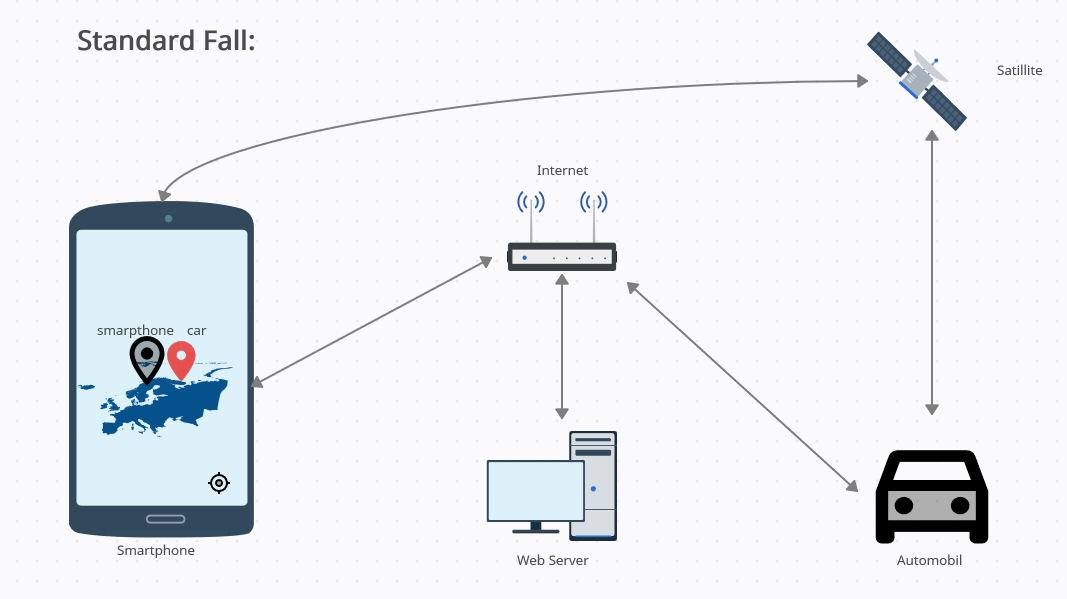
\includegraphics[width=1\textwidth]{Bilder/StandardFall.PNG}
            \caption{Konzept der Android App im Standard Fall}
            \label{alarmfall}
\end{figure}
\subsubsection{Alarm Fall} 
Im Falle das sich der Standort des Automobils ändert, wird ein Alarm auf dem Handy ausgelöst und der Nutzer bekommt eine Push-Benachrichtigung.
     \begin{figure}[H]
            \centering
            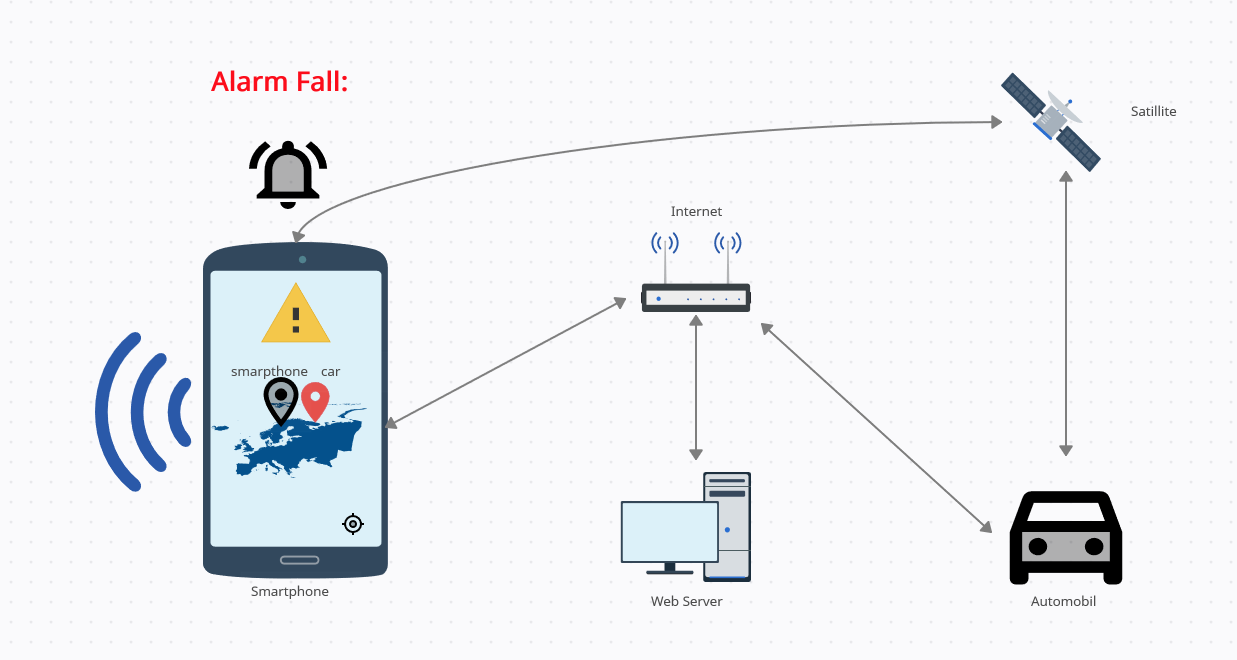
\includegraphics[width=1\textwidth]{Bilder/AlarmFall.PNG}
            \caption{Konzept der Android App im Alarm Fall}
            \label{standardfall}
	
    \end{figure}
	
\subsection{Implementierung}
\subsubsection{Flutter Funktionalität}
Flutter ist sehr einfach zu verstehen und verkürzt die Lernkurve erheblich. Die Grundidee lautet: “Alles ist ein Widget“. Es ist dem Entwickler völlig selbst überlassen, wie er sein Projekt
strukturieren und hinsichtlich Architektur- und Entwurfsmuster logisch aufbauen möchte. Der Einstiegspunkt zu Flutter ist die main.dart-Datei oder die zentrale main()-Methode. Von dort aus ist es möglich, sich gegenseitig zu verschachteln und zu importieren.
Die Entwicklung von Flutter beinhaltet hauptsächlich nur Widgets, weil alles hineingeschrieben wird.
Sogar ein einfacher Text “Teil“ wird als Widget festgelegt.
\\\\
In Flutter gibt es ebenfalls eine Baumstruktur \textit{“Widget Tree“}. Jede betriebssystemspezifische Komponente, die man in Flutter verwenden möchte, muss zunächst von einem Flutter-Entwickler nativ entwickelt werden. Dies ist jedoch nur dann erforderlich, wenn die Anwendung auch der nativen Anwendung ähnlich sein soll.
Aus den Basis-Komponenten, der verschiedenen Pakete, konnte man eigene Widgets schreiben. So kann sich ein eigener, abgerundeter Button beispielsweise durch eine Kombination aus RawMaterialButton, Text und Icon-Widgets darstellen lassen.
In Flutter werden Widgets  als einfache Klassenvariablen über den Konstruktor der Klasse übergeben und können dort beliebig verwendet werden.
Durch die Klassenvariablen lassen sich Komponenten in
ihrem Aussehen sowie ihrer Funktionalität individualisieren und anpassen \cite{SDK}.\\\\
Es gibt zwei Arten von Komponenten in Flutter, die im Code explizit als solche benannt werden. Erstens  \textit{“Statful-Widgets“}, die einen Zustand beibehalten oder verwalten können. Andererseits gibt es \textit{“Stateless Widgets“}, die nur als statische, einfache Widgets dienen. Ein zustandsbehaftetes Widget erfordert immer eine zugeordnete createState()-Funktion. Eine Methode, die ein Zustandsobjekt (\textit{private Klasse}) erstellt, welche wiederum
den Widget-Status verwaltet. Abgesetzt durch Aufruf von setState()
ruft die Methode build() auf, um die Komponente neu zu zeichnen. Die build()-Methode wird bei dem Umwandeln eines Stateless Widgets in ein Stateful Widget, in die private State-Klasse ausgelagert.\\\\
Das Styling in Flutter ist grundlegend speziell. Wenn man das Widget zentrieren möchten, könnte man beispielsweise das Center-Widget verwenden.
Um ein Widget von anderen Widgets zu entfernen, muss es dafür mit einem Padding-Widget umschlossen werden. Als einfaches Beispiel kann ein Text-Widget von einem Center-Widget umgeben werden, welche wiederum von einem Container-Widget umgeben sind.\\\\
“Center“, “Raw“, “Column“, “Container“-Widgets und viele andere Widgets
sind die Bausteine in der Entwickelung von Flutter App.
\subsection{Implementierung SchrödingersAlarm App}
\subsubsection{Login Menü}
Das Starten der App ist hier Standard, wie bei jeder App. Zuerst kommt die Willkommensseite, in der ein Login Menü erscheint.
Jedes Alarmsystem soll eine eigene IMEI und dazugehörigen PIN Code haben und den Kunden mitgeliefert werden.
Diese beiden Informationen sind in der Datenbank  der App hardcodiert eingefügt, da dieses Feature noch aussteht. 
Das Logo des Produkts wird oben angezeigt und unten sind zwei Eingabefelder definiert,
in denen man die Login-Informationen(IMEI/PIN) eingeben kann. Der Login-Prozess hat einen genau definierten Mechanismus. In den beiden Feldern muss eine bestimmte Anzahl an Zeichen eingegeben werden, ansonsten wird es nicht akzeptiert. Die IMEI muss 15 Ziffern beinhalten. Der PIN Code muss 6 Ziffern beinhalten. Nur bei einer korrekten Dateneingabe wird man zu der nächsten Seite geleitet.
Andernfalls erscheint eine rote Fehlermeldung, die um korrekte Informationen bittet.\\\\
Wie vorher beschrieben ist, wird die Horizontale aufgeteilt. Der obere Teil ist das importierte Bild vom Logo und im unteren Teil sind die genannten Eingabefelder, siehe Abbildung \ref{login}]
Diese Aufteilung wird mit einem “Column“ Widgets definiert. Der unter Teil wird ebenfalls in viele Widgets aufgeteilt.


 \begin{figure}[H]
            \centering
            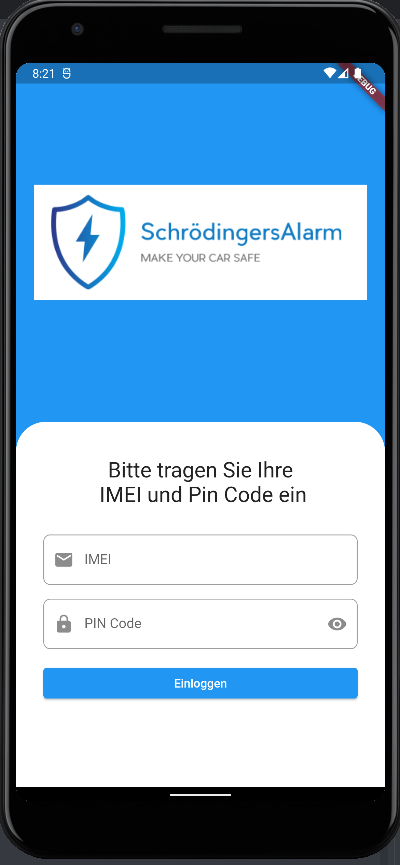
\includegraphics[width=0.4\textwidth]{Bilder/LoginIn.PNG}
            \caption{Android App \textit{Login Seite}}
            \label{login}
    \end{figure}

\subsubsection{Hauptseite}
Nach erfolgreichem Login leitet die App den Nutzer auf die Hauptseite.
Auf der Hauptseite gibt es eine horizentale Appbar mit 3 Kategorien (\textit{Home/Status/Maps}), links oben ein Menu Item für Support und rechts oben ein Logout item für das Ausloggen aus der App.
Im Hometab wird das Logo und der aktuelle Standort angezeigt.
Ist die App aktiviert, wird ein grüner Kreis mit der Meldung \textit{“your car is safe“} angezeigt.
Ist sie deaktiviert, wird ein roter Kreis mit der Meldung \textit{“Dangerous situation“} ausgegeben.\\\\
Durch das Drücken auf „Status“ in der horizontalen Appbar, werden die Informationen, die vom Webserver kommen, in einem Text Widget angezeigt.
Wichtig ist hier, auf eine Webserver Verbindung zu prüfen. Besteht eine Verbindung, soll ein grünes Verbindungs-Icon angezeigt werden, andernfalls ein  Icon “Nicht verbunden“.\\\\
Das dritte Item in der horizontalen Appbar ist die Karte. In dieser wird die Google Maps Anwendung in der App geöffnet.
Die Koordinaten, die von dem Webserver kommen, werden dann mit einem Marker in der Google Maps Karte markiert, wie in Abbildung \ref{seiten} zu sehen. 
Dazu kommt der gespeicherten Parking Standort in einem anderen Marker angezeigt.\\\\
Falls die Koordinaten vom Webserver zu sehr von den gespeicherten Koordinaten abweichen, bekommt der Nutzer eine Push-Benachrichtigung. Bei der Umrechnung werden Longtitude und Latitude von beiden Koordinaten abgezogen und die Differenz berechnet.
Falls einer der beiden Werte höher als der festgelegten Wert ist, erstellt die App eine Push-Benachrichtigung.
 	\begin{figure}[H]
   \centering
            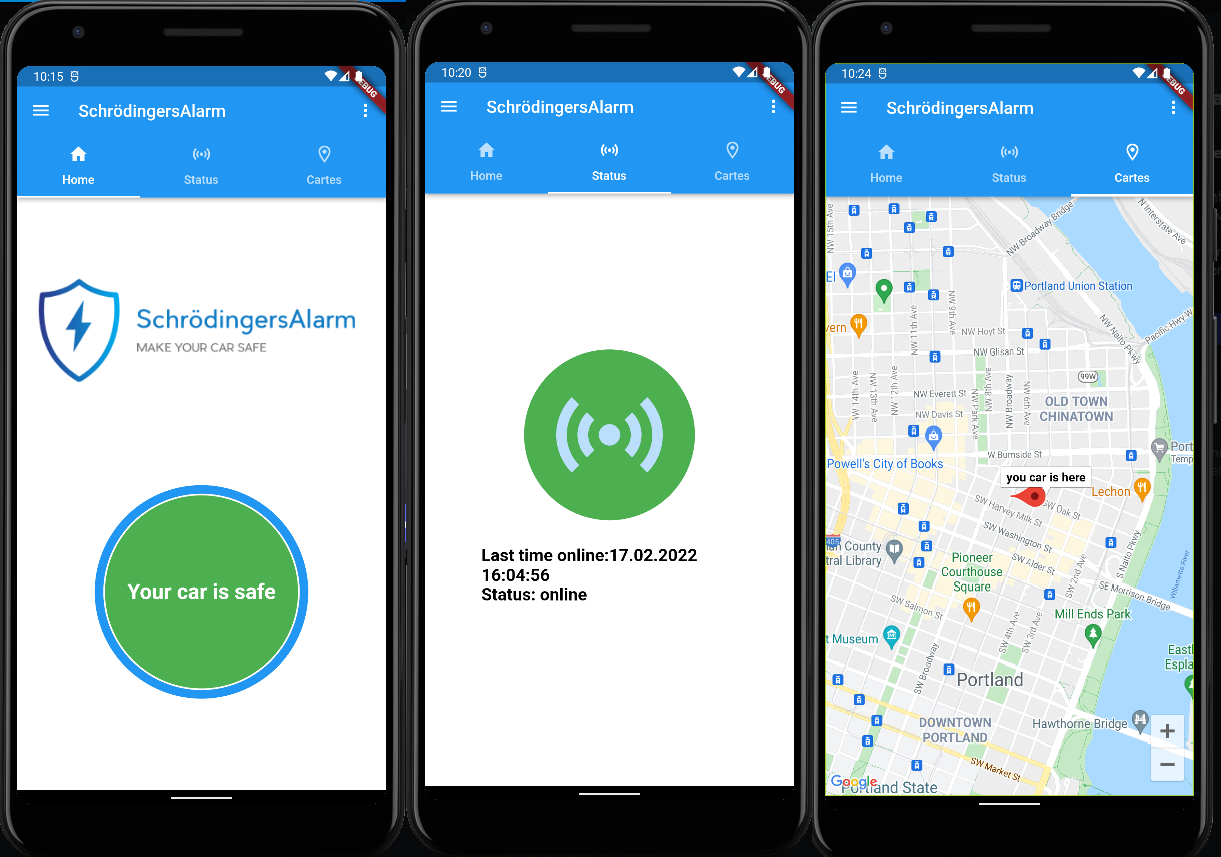
\includegraphics[width=1\textwidth]{Bilder/hauptseite.PNG}
		            \caption{Android App \textit{Seitenanichten}}
		            \label{seiten}
    \end{figure}
